\section{Bài toán}\label{sec:bai-toan}

\subsection{Hệ thống và camera}

Drone S500 của nhóm bay bằng ArduPilot và mang một bo camera riêng: ESP32-S3 N16R8 với cảm biến OV3660, gắn nhìn thẳng xuống đất. Bo nối Mobile Hotspot của laptop và phát luồng MJPEG qua HTTP, mỗi khung là một ảnh JPEG 640$\times$480 nén ở mức chất lượng 12 của ESP32. Ngoài bãi bay, luồng đạt 2 đến 9 khung/s tuỳ khoảng cách và tình trạng Wi-Fi. Mọi xử lý AI chạy trên laptop (GPU RTX 4060 Laptop 8 GB) chứ không chạy trên drone, vì bo ESP32-S3 chỉ đủ sức nén và gửi ảnh. Hình~\ref{fig:pipeline} là đường đi của một khung từ cảm biến tới màn hình người vận hành.

\begin{figure}[!htbp]
\centering
\begin{tikzpicture}[
  font=\scriptsize, node distance=4mm and 5mm,
  khoi/.style={draw=#1, fill=#1!12, rounded corners=2pt, line width=0.8pt, align=center, minimum height=12mm, text width=21mm},
  mui/.style={-{Stealth[length=2.2mm]}, line width=0.9pt, cXam},
]
\node[khoi=cHong] (cam) {\textbf{Camera}\\ESP32-S3 N16R8\\+ OV3660\\JPEG 640$\times$480, q12};
\node[khoi=cVang, right=of cam] (wifi) {\textbf{Wi-Fi}\\Mobile Hotspot\\MJPEG qua HTTP\\2–9 khung/s};
\node[khoi=cXanh, right=of wifi, text width=25mm] (gcs) {\textbf{Laptop, backend}\\FastAPI, ONNX Runtime\\CUDA, RTX 4060 Laptop\\giải mã 0,7 ms};
\node[khoi=cCam, above right=1mm and 6mm of gcs.east, anchor=south west, text width=28mm] (det) {\textbf{Detector ONNX}\\YOLO11s, letterbox 1280\\khung gốc, bỏ 16 cột\\23,6 ms p50};
\node[khoi=cTim, below right=1mm and 6mm of gcs.east, anchor=north west, text width=28mm] (enh) {\textbf{Enhancer ONNX}\\NAFNet-w16\\chỉ khi có người xem\\12,5 ms p50};
\node[khoi=cLuc, right=39mm of gcs, text width=18mm, minimum height=26mm] (web) {\textbf{Web React}\\hộp người,\\cảnh báo,\\luồng ``Ảnh rõ''};
\node[draw=cXam, dashed, rounded corners=2pt, fill=cXam!6, align=center, text width=30mm, below=3mm of enh] (cls) {Chuỗi lọc cổ điển\\CPU 9,2 ms (trong XLA)};
\draw[mui] (cam) -- (wifi);
\draw[mui] (wifi) -- (gcs);
\draw[mui] (gcs.east) -- ++(3mm,0) |- (det.west);
\draw[mui] (gcs.east) -- ++(3mm,0) |- (enh.west);
\draw[mui] (det.east) -| ($(web.north west)!0.35!(web.north east)$);
\draw[mui] (enh.east) -| ($(web.south west)!0.35!(web.south east)$);
\draw[cXam, dashed, line width=0.6pt] (cls.north) -- (enh.south);
\end{tikzpicture}

\caption[Đường đi của một khung ảnh]{Đường đi của một khung ảnh. Nhận diện luôn chạy trên khung gốc; ảnh rõ chỉ phục vụ người xem. Bộ lọc cổ điển chạy trong XLA, chưa nằm trong hợp đồng model của IOT-CV.}
\label{fig:pipeline}
\end{figure}

Đồ án có hai đầu ra trên cùng một khung đầu vào (JPEG 640$\times$480, BGR, chưa qua xử lý):
\begin{itemize}
\item \textbf{nhận diện:} các hộp $[x_1,y_1,x_2,y_2]$ kèm độ tin cậy cho lớp người, theo toạ độ của chính khung đó, để web cảnh báo người vận hành;
\item \textbf{ảnh rõ:} một khung cùng cỡ, dễ nhìn hơn cho người ngồi trước laptop.
\end{itemize}
Bài toán dùng kiến thức các chương biểu diễn ảnh, nâng cao chất lượng, hệ màu, nén JPEG và nhận dạng của học phần~\cite{baigiang,gonzalez}. Luật đặt ra từ đầu: điểm số chỉ chấm trên khung bay thật. Ảnh tự sinh dùng để huấn luyện được, nhưng không dùng để kết luận model nào tốt hơn. Nhóm đặt hai câu hỏi nghiên cứu: (1) làm xấu ảnh huấn luyện theo số đo của chính camera này (D2) có cho bộ nhận diện tốt hơn làm xấu ngẫu nhiên (D1) trên khung thật không; (2) làm rõ ảnh trước khi nhận diện có giúp bộ nhận diện không.

\subsection{Camera này làm hỏng ảnh ở đâu}

Nhóm đo hồ sơ camera trên 1\,115 khung dev của chuyến bay 02/11/2026 (bản ghi \texttt{20261102-100941}); khung test không tham gia. Bảng~\ref{tab:camera} liệt kê năm lỗi chính, Hình~\ref{fig:loi-camera} cho thấy chúng trên khung thật. Lỗi nặng nhất là ám hồng: khi điểm ảnh gần bão hoà, kênh G bị cắt ở mức thấp hơn R và B, nên đường bê tông và mái tôn sáng biến thành mảng hồng. Hồ sơ này là nền của mọi bước sau: bộ làm xấu D2 đọc thẳng số đo từ nó, bộ lọc cổ điển bù tối góc theo tiêu cự trong nó, và web IOT-CV nén khung giả bằng chính bảng lượng tử đo được.

\begin{table}[!htbp]
\centering\footnotesize
\caption[Lỗi ảnh đo trên 1\,115 khung dev]{Lỗi ảnh đo trên 1\,115 khung dev (hồ sơ \texttt{ov3660-esp32s3-q12-20261102}, bản 1.2.0). Số là trung vị, ngoặc là p5–p95.}
\label{tab:camera}
\begin{tabularx}{\textwidth}{@{}l X l@{}}
\toprule
Lỗi & Đại lượng đo & Giá trị \\
\midrule
Ám hồng vùng sáng & tỉ lệ điểm có $R-G>25$ và $B-G>25$; khung có $>0{,}5\,\%$ điểm hồng & 0,17\,\% (0–3,3\,\%); 31\,\% số khung \\
Mù như sương & dark channel, ô 15 px (thang 0–255) & 143,7 (134,6–152,1) \\
 & độ bão hoà màu (0–255) & 16,2 (7,5–22,7) \\
Vỡ khối JPEG & tỉ số biên khối $8\times8$; bảng DQT & 2,68 (2,15–3,52); Annex K $\times$ 0,75, 4:2:2 \\
Tối góc & tỉ số sáng góc/tâm; tiêu cự khớp mô hình $\cos^4$ & 0,81 (0,62–0,93); 1\,016 px \\
Dải tối mép trái & bề rộng dải; độ sáng Y trong dải & 14 px (13–16); 100,9 so với nền 152,3 \\
Nhoè & phương sai Laplacian; $\sigma$ PSF Gauss khớp từ MTF50 & 34,1 (13,4–67,4); 0,76 px \\
\bottomrule
\end{tabularx}
\end{table}

\begin{figure}[!htbp]
\centering
\begin{subfigure}[b]{0.43\textwidth}\centering
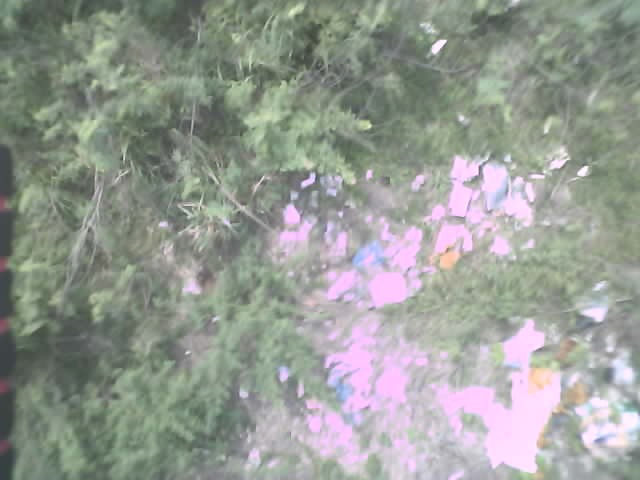
\includegraphics[width=\linewidth]{fig/art_full.jpg}
\caption{Khung \texttt{004\_01252}: mảng hồng, mù, tối góc}\end{subfigure}\hfill
\begin{subfigure}[b]{0.30\textwidth}\centering

\includegraphics[width=\linewidth]{fig/art_pink.jpg}
\caption{Mảng hồng phóng 4$\times$, thấy rõ khối 8$\times$8}\end{subfigure}\hfill
\begin{subfigure}[b]{0.105\textwidth}\centering
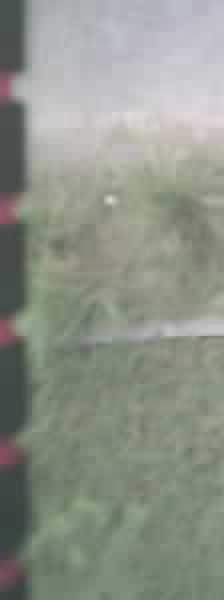
\includegraphics[width=\linewidth]{fig/art_strip.jpg}
\caption{Dải mép}\end{subfigure}\hfill
\begin{subfigure}[b]{0.13\textwidth}\centering

\includegraphics[width=\linewidth]{fig/art_block.jpg}
\caption{Biên khối, 8$\times$}\end{subfigure}
\caption[Lỗi của camera trên khung bay thật ngày 02/11/2026]{Lỗi của camera trên khung bay thật ngày 02/11/2026. Dải mép (c) là khối tối xen vạch đỏ đều, chu kỳ 60 px, rộng khoảng 14 cột; mọi model đều bỏ 16 cột đầu.}
\label{fig:loi-camera}
\end{figure}
